\section{Image-Based Applications}

All applications use $\theta_{\mathrm{mask}}=10^{-3}$ and fixed
$a_{\mathrm{surf}}^{\mathrm{interface}}+a_{\mathrm{surf}}^{\mathrm{intrinsic}}$.
Online Resource~1 provides image, grid, transport, surface-reaction,
concentration, runtime, and MPI specifications for result-supporting cases.

\subsection{Pb$^{2+}$ Uptake in a Two-Dimensional Fracture Network}

The \nolinkurl{4StraightFractures} image contains microporous matrix and open
fractures on a $250\times250\times1$ computational grid. Pb$^{2+}$ enters at
$10^{-3}$~mol\,L$^{-1}$ and equilibrates with strong and weak
Dzombak--Morel HFO sites \citep{dzombak1990surface}. The reactive-area field
combines the reconstructed matrix--fracture interface with
$10^5$~m$^{-1}$ of intrinsic area in the matrix, whose end-member porosity is
$0.4$.

At $t=20000$~s, dissolved Pb$^{2+}$ preferentially follows the connected
fractures while strong-site occupancy extends into the adjacent microporous
matrix (Figure~\ref{fig:2DFractures}). Uptake is greatest near the inlet and
fracture intersections, where advective delivery and matrix area coincide.
The result illustrates the central scale separation: open cells control rapid
delivery, whereas unresolved matrix area controls much of the adsorbed
inventory.

The paired fields distinguish transport access from sorption capacity. The
dissolved field follows the connected fracture network because those cells
carry the rapid flow paths. Strong-site occupancy persists in matrix cells
adjacent to the fractures because the matrix retains mobile water and the
specified intrinsic area. Thus the spatial pattern is not interpreted as a
direct image of velocity: it reflects the overlap of delivered Pb$^{2+}$,
accessible microporous water, and local HFO capacity.

\begin{figure}[htbp]
    \centering
    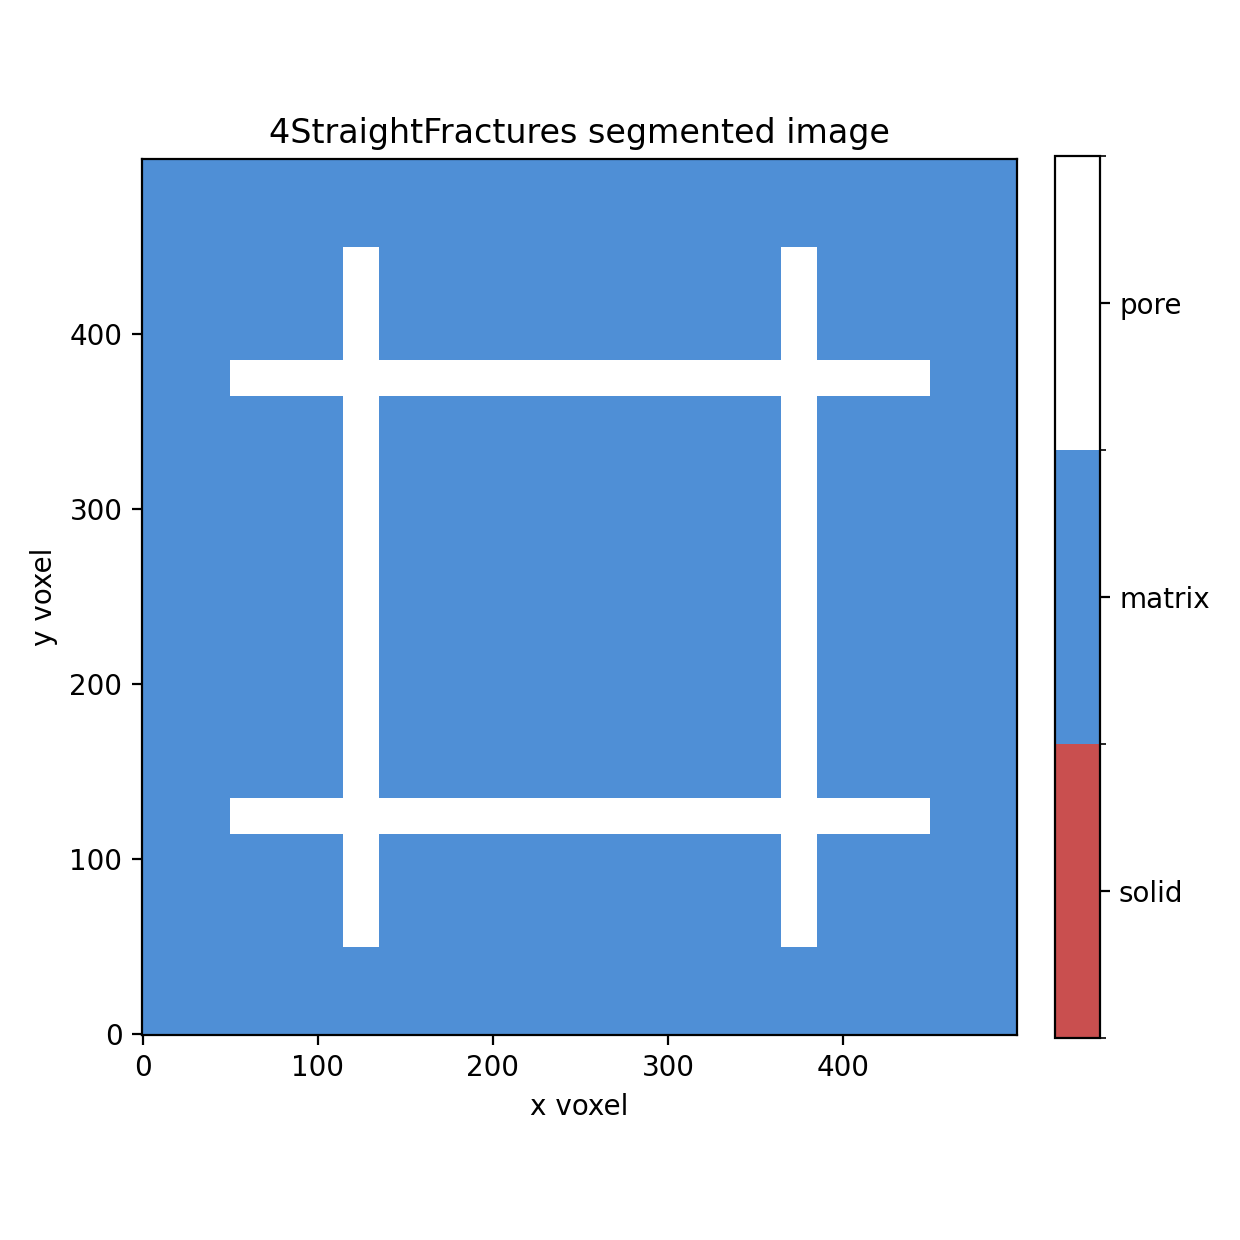
\includegraphics[width=0.82\linewidth]{figures/png/fig02_2d_fractures.png}
    \caption{Pb$^{2+}$ transport and HFO occupancy at $t=20000$~s. From left:
    segmented fracture geometry, dissolved $\mathrm{Pb}^{2+}/C_{\mathrm{in}}$
    with logarithmic colour normalisation, and strong-site occupancy with
    logarithmic colour normalisation. Zero-area cells are masked in the
    occupancy panel.}
    \label{fig:2DFractures}
\end{figure}

\subsection{Sr$^{2+}$/Ca$^{2+}$ Exchange in Estaillades Limestone}

The large application uses a $500^3$ three-phase Estaillades image with
$4~\mu$m voxels \citep{menke2021upscaling}. Open pore, micropore, and solid
labels are represented at native resolution. Micropores carry $\theta=0.4$
and intrinsic area $10^5$~m$^{-1}$. A $10^{-4}$~mol\,L$^{-1}$ Sr$^{2+}$
inlet displaces an initially equilibrated $10^{-3}$~mol\,L$^{-1}$ Ca$^{2+}$
solution from \texttt{Surf\_a} sites; the Sr reaction has the slightly larger
equilibrium constant ($\log K=-5.5$ versus $-5.85$ for Ca).

The image produces chromatographic exchange rather than single-species
retardation. Sr$^{2+}$ adsorption advances behind a Ca$^{2+}$ desorption wave,
and loading follows the connected reactive microporosity
(Figure~\ref{fig:3DEstaillades}). Across the saved checkpoints from 0 to
120~s, the porosity-weighted mean Sr$^{2+}$ concentration rises to $0.865$
$C_{\mathrm{in}}$, while Ca$^{2+}$ falls from $1.000$ to $0.095$
$C_{\mathrm{init}}$. Surface-area-weighted \texttt{Surf\_aSr+} increases
monotonically as \texttt{Surf\_aCa+} decreases
(Figure~\ref{fig:EstailladesTemporal}); the signed changes are referenced to
$t=0$ and divided by the largest absolute change across both surface species
and all plotted times. This directly identifies replacement of
resident Ca by invading Sr.

The temporal and spatial views provide complementary evidence for this
interpretation. The volume rendering shows where the invading dissolved Sr and
its surface loading occur in the connected image, whereas the weighted time
series shows the opposing changes in the Sr and Ca inventories. The Ca decrease
is therefore associated with competitive displacement from the fixed surface
state, rather than being inferred solely from the aqueous front. These
application results illustrate the consequence of representing the internal
microporous area as capacity; they do not independently determine its physical
magnitude.

\begin{figure}[htbp]
    \centering
    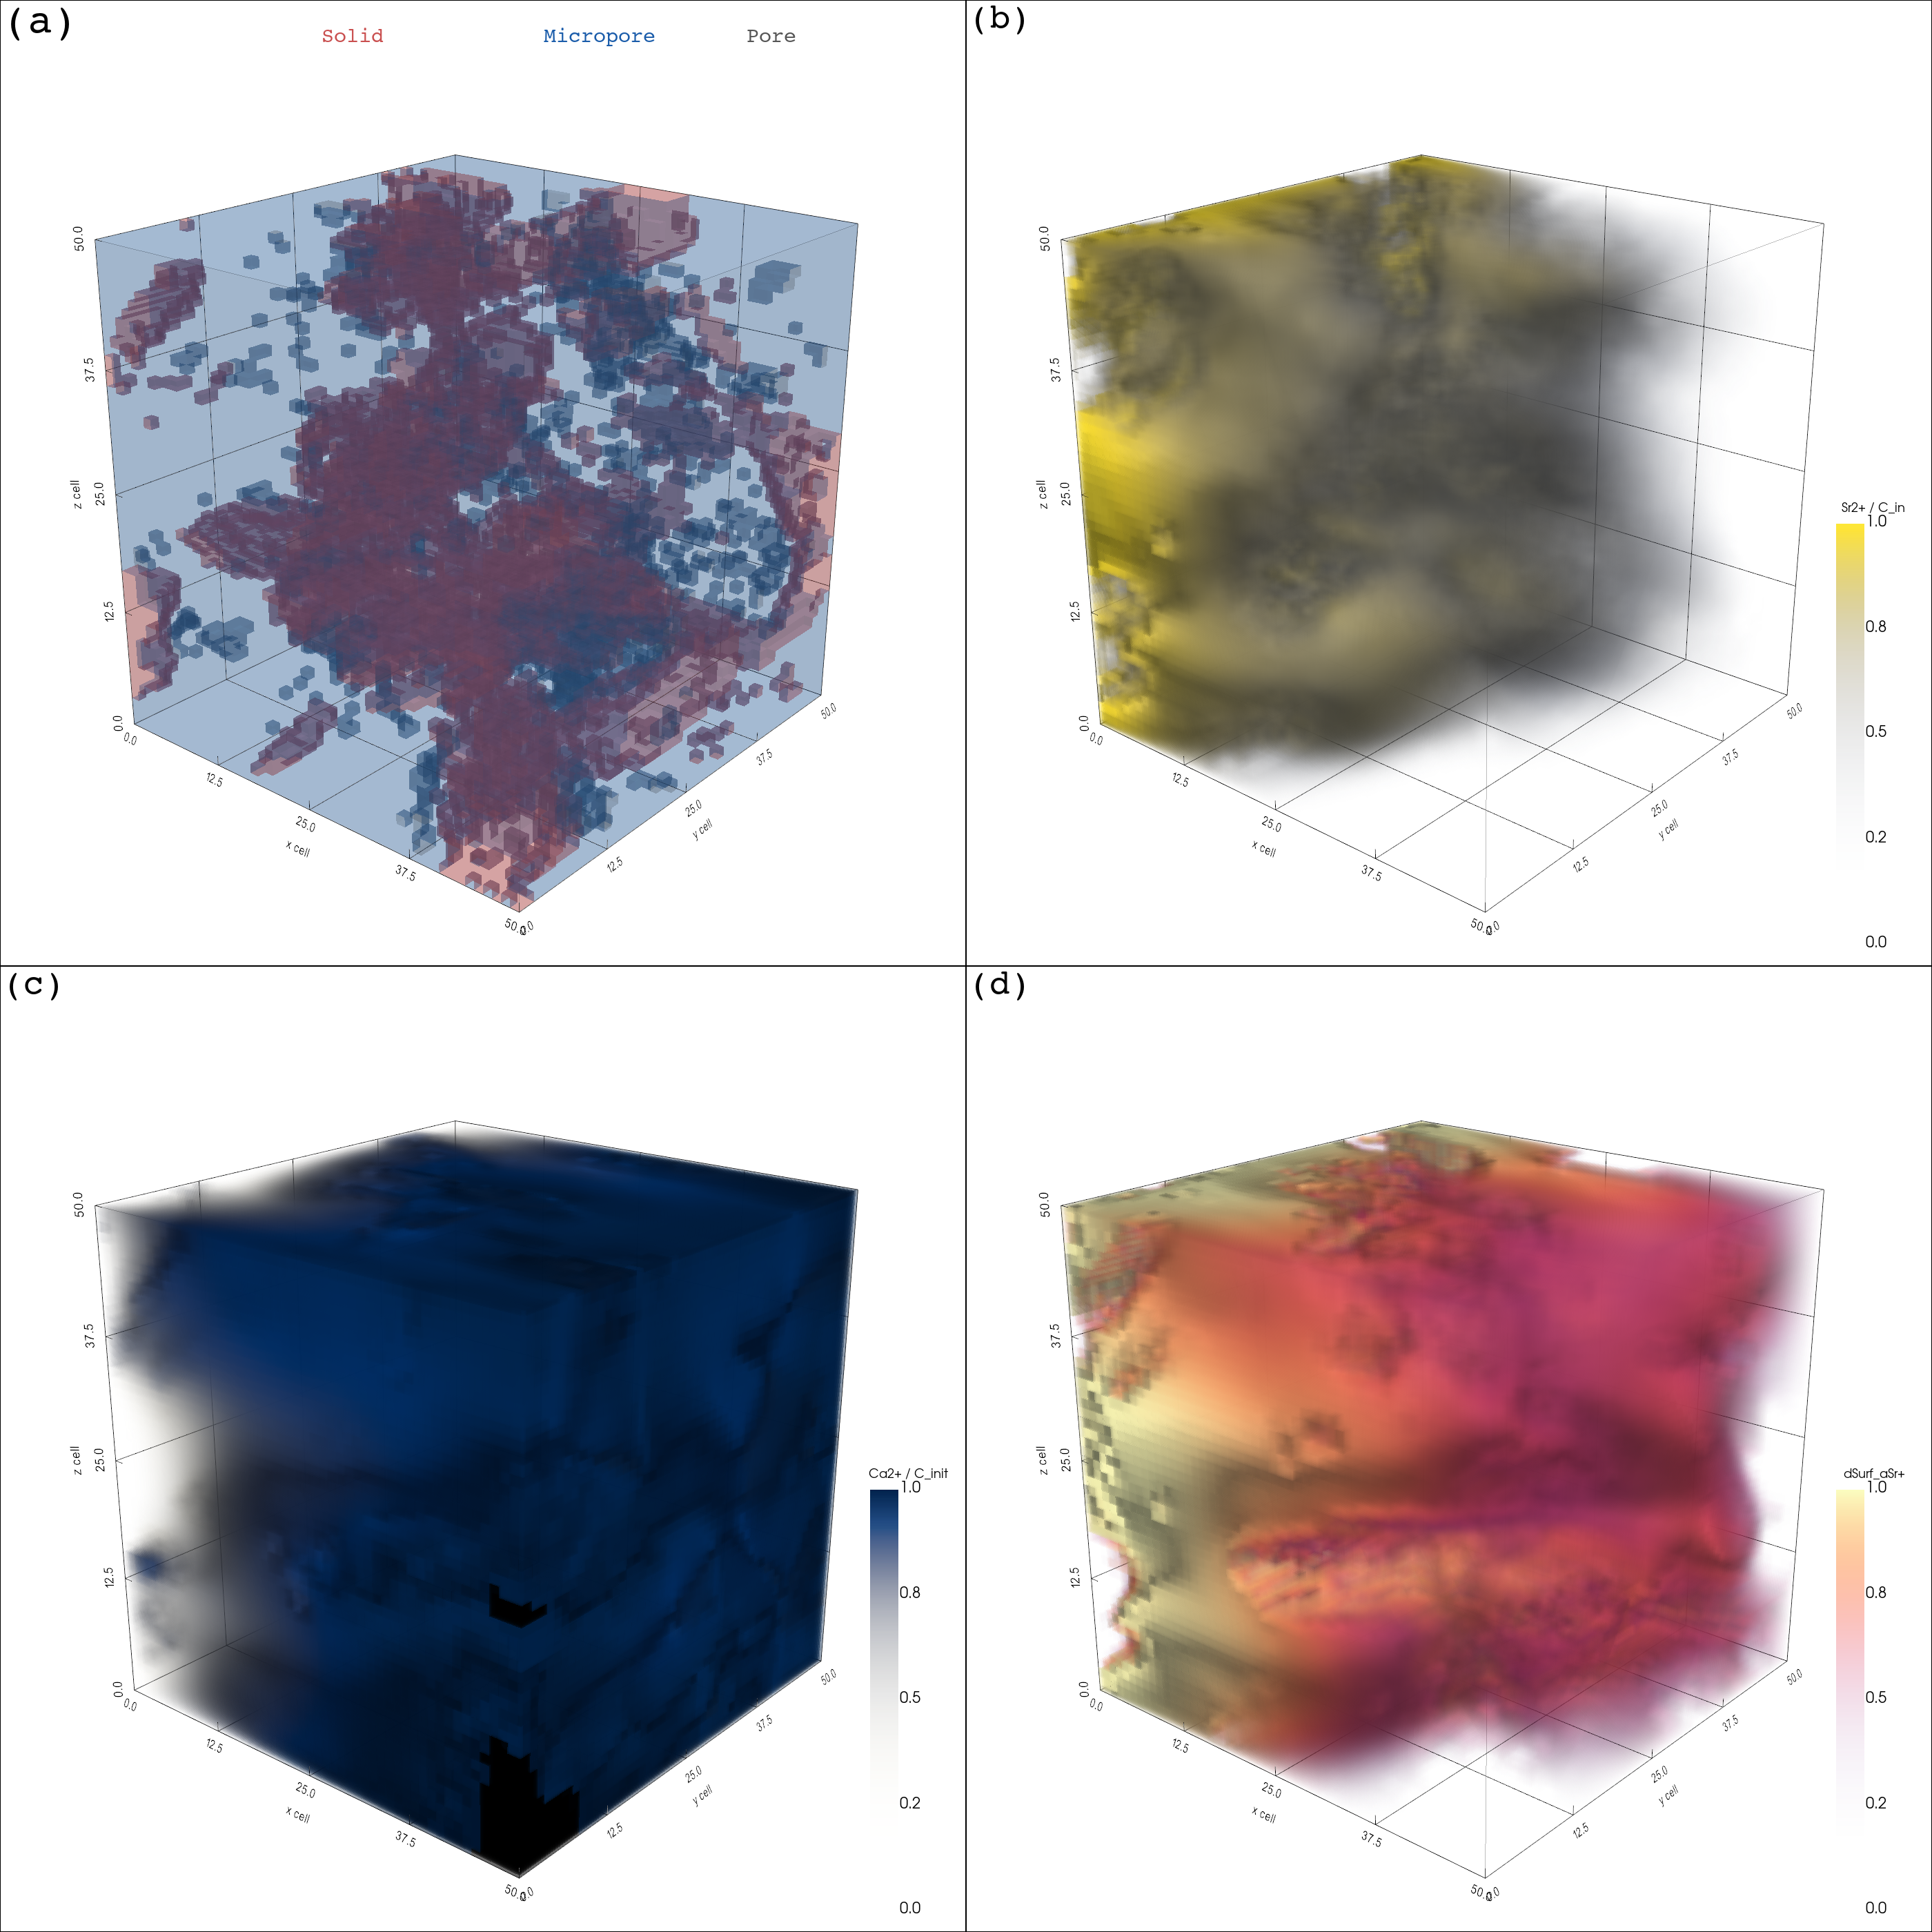
\includegraphics[width=\linewidth]{figures/png/fig04_3d_estaillades.png}
    \caption{Estaillades exchange at $t=40$~s. Panels show the segmented
    geometry, dissolved Sr$^{2+}/C_{\mathrm{in}}$ and
    Ca$^{2+}/C_{\mathrm{init}}$, and the incremental adsorbed Sr$^{2+}$
    loading relative to $t=0$, normalised by its maximum at 40~s. The plume
    enters from the left and loads the distributed microporous surface.}
    \label{fig:3DEstaillades}
\end{figure}

\begin{figure}[htbp]
    \centering
    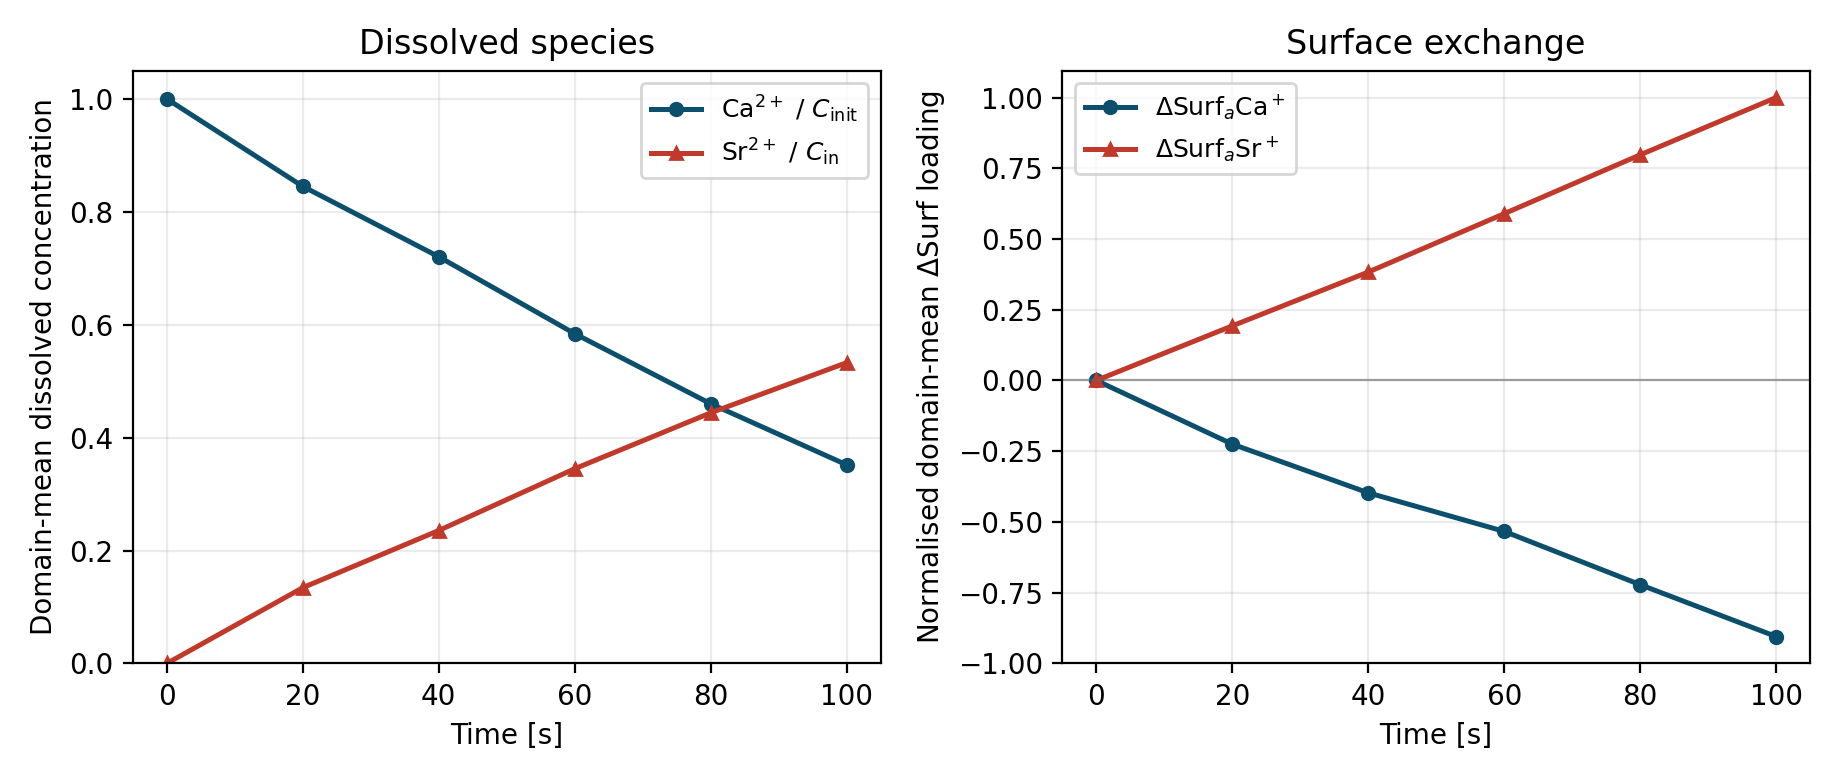
\includegraphics[width=0.86\linewidth]{figures/png/fig08_estaillades_temporal.png}
    \caption{Estaillades exchange from 0 to 120~s. Porosity-weighted dissolved
    Ca$^{2+}$ and Sr$^{2+}$ (left) are paired with signed changes in
    surface-area-weighted adsorbed amounts (right). Each surface change is its
    value minus that at $t=0$, divided by the largest absolute change across
    both species and all plotted times, showing Sr invasion and Ca displacement
    in both inventories.}
    \label{fig:EstailladesTemporal}
\end{figure}
